\chapter{Motivation}

Prototyping, design evaluation, and the measurement of physical properties in experiments make a daily occurrence in the engineering praxis. Those tasks often involve the generation and sampling of electrical signals coming to and from sensors, actuators, and other circuitry.

Recently, a wide range of intelligent sensors became available thanks to the drive to miniaturization in the consumer electronics industry (\cref{fig:some_sensors}). Those devices often provide sufficient accuracy and precision while keeping the circuit complexity and cost low. In contrast to analog sensors, here the signal conditioning and processing circuits are built into the sensor itself, and we access it through a digital connection.

\begin{figure}[H]
	\centering
	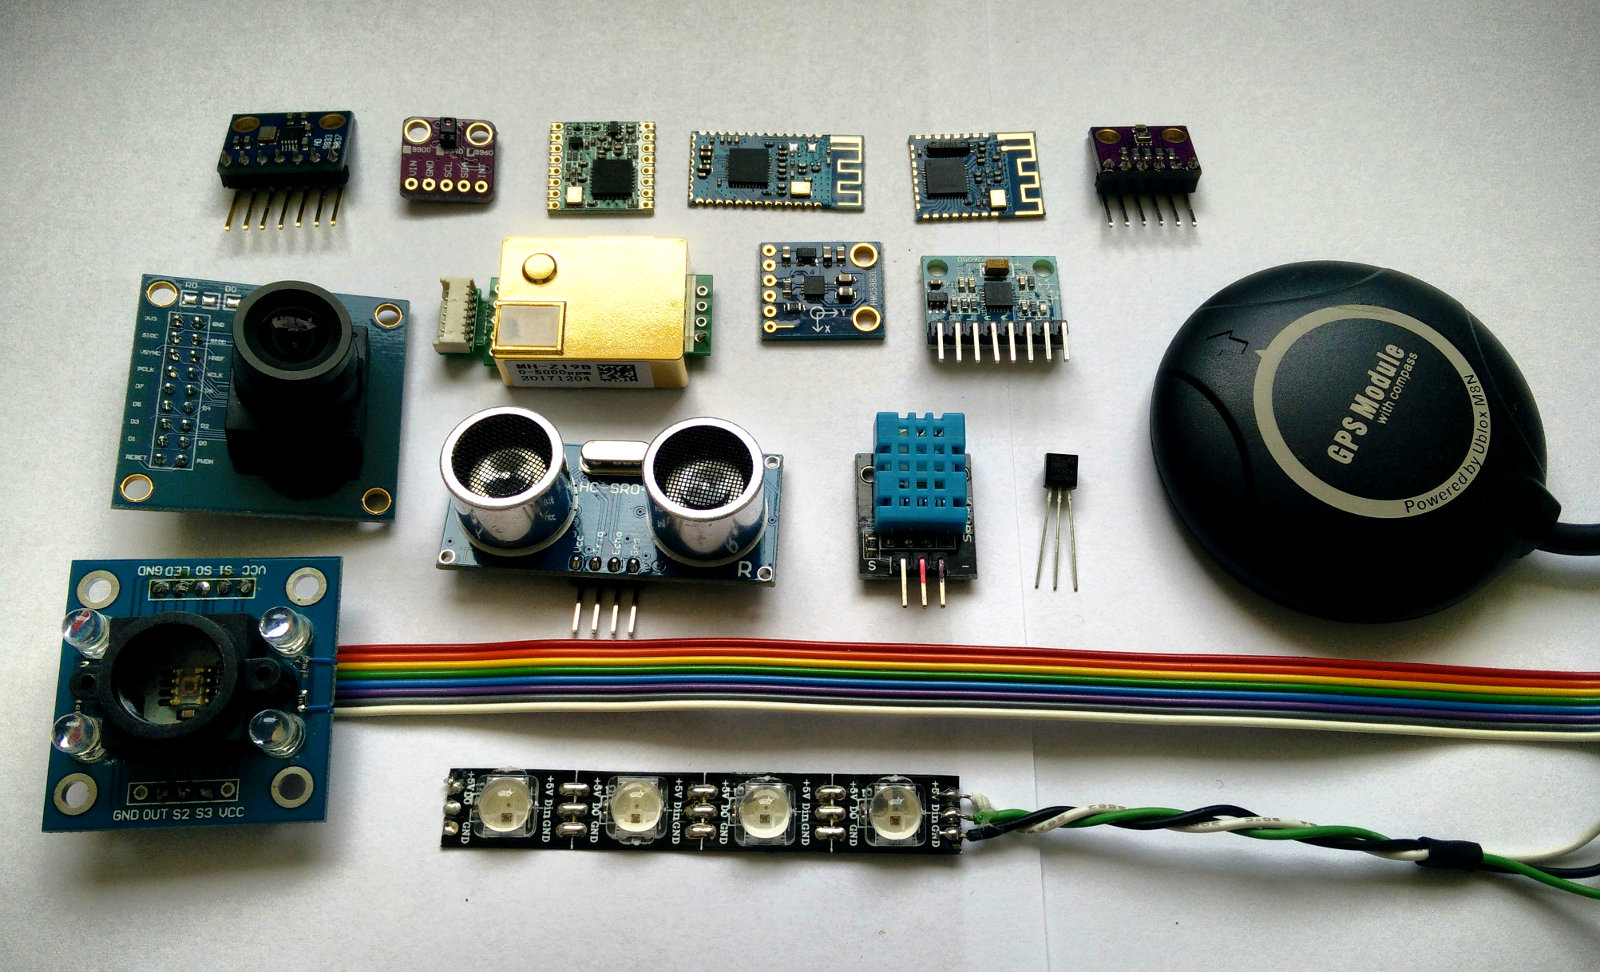
\includegraphics[width=0.8\textwidth] {img/inteligent-sensors.jpg}
	\caption[A collection of intelligent sensors and devices]{\label{fig:some_sensors}A collection of intelligent sensors and devices, most on breadboard adapters: (from the top left) a waveform generator, a gesture detector, a LoRa and two Bluetooth modules, an air quality and pressure sensor, a CO$_2$ sensor, a digital compass, an accelerometer, a GPS module, a camera, an ultrasonic range finder, a humidity sensor, a 1-Wire thermometer, a color detector, and an RGB LED strip}
\end{figure}

If we wish to conduct experiments with these integrated modules, or just familiarize ourselves with a device before using it in a project, we need an easy way to interact with them. It would also be convenient to have direct access to low-level hardware, be it analog signal sampling, generation, or even just the access to logic inputs and outputs. However, advances in computer technology, namely the advent of the \gls{USB}, lead to the disappearance of low-level computer ports, such as the printer port (LPT), that would provide an easy way of doing so.

Today, when we want to perform measurements using a digital sensor, the usual route is to implement embedded firmware for a microcontroller that connects to the \gls{PC} through \gls{USB}, or perhaps shows the results on a display. This approach has its advantages, but is time-consuming and requires specific knowledge unrelated to the measurements we wish to perform. It would be advantageous to have a way to access hardware without having to burden ourselves with the technicalities of this connection, even at the cost of lower performance compared to specialized devices or professional tools.

The design and implementation of such a universal instrument is the object of this work. For technical reasons, such as naming the source code repositories, we need a name for the project; it shall be hereafter called \textbf{GEX}, a name derived from ``\textbf{G}PIO \textbf{Ex}pander''.

\section{Expected Outcome}\label{sec:expected_outcome}

It has been a long-time desire of the author to create a universal instrument connecting low-level hardware to a computer, and, with this project, it is finally being realized. Several related projects approaching this problem from different angles can be found on the internet; some of these will be presented in \cref{sec:prior_art}. 

Our project is not meant to end as a tinkering tool that will be produced in a few prototypes and then forgotten. By creating an extensible, open-source platform, GEX can become the foundation for future projects which others can expand, re-use, and adapt to their specific needs.

\iffalse
\begin{figure}[H]
	\centering
	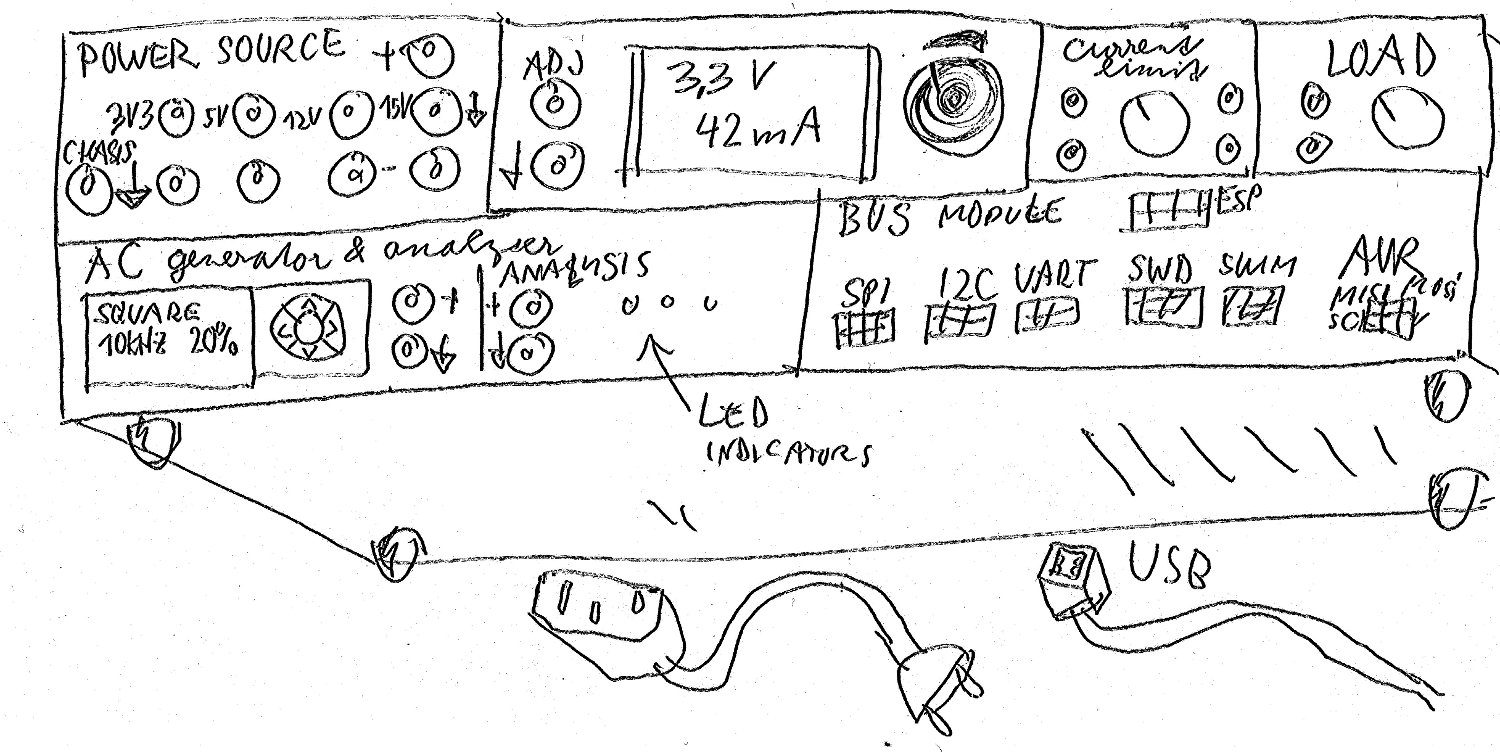
\includegraphics[width=0.7\textwidth] {img/early-sketch.jpg}
	\caption[An early sketch of a universal bench device]{An early (2016) sketch of a universal bench device including a power supply, electronic load, a signal generator and a bus module. The bottom half of the panel is in a large part implemented by GEX.}
\end{figure}
\fi

Building on the experience with earlier embedded projects, an STM32 microcontroller will be used. Those are \armcm devices with a wide range of hardware peripherals that should be a good fit for the project. Low-cost evaluation boards are available that could be used as a hardware platform instead of developing a custom \gls{PCB}. STM32 microcontrollers are affordable and already popular in the embedded hardware community, so there is a real possibility of the project gathering a community around it and growing beyond what will be presented in this paper.

\iffalse
Besides the use of existing development boards, custom \glspl{PCB} will be developed in different form factors. The possibilities of wireless connection should be evaluated. This feature should make GEX useful for instance in mobile robotics or when installed in poorly accessible locations.
\fi







